% -*-coding: utf-8;-*-
% $Id: Part1_New.tex,v 1.5 2008-01-28 10:58:34 evlad Exp $
%%%%%%%%%%%%%%%%%%%%%%%%%%%%%%%%%%%%%%%%%%%%%%%%%%%%%%%%%%%%%%%%%
% Глава 1 - Обзор литературы

\section{Области применения нейронных сетей в современных системах
         управления}%

%%% Вводная

Системы автоматического управления являются критически важной и
неотъемлемой частью современных технических устройств, комплексов и
процессов.  Тенденции развития цивилизации таковы, что сама
жизнедеятельность человека становится все более зависимой от
нормального функционирования технических систем, а значит, от систем
управления ими.

Развитие современных систем управления характеризуется следующими
ключевыми аспектами~\cite{kulee96}:

\begin{itemize}

\item
Возрастающая сложность управляемых объектов и систем управления ими.

\item
Повышение требований к темпам разработки.

\item
Удовлетворение приведенных выше требований меньшими и менее точными
знаниями об объекте управления и его окружении.

\end{itemize}

Для решения возникающих все более сложных задач управления аппарат
теории управления развивается как вглубь (совершенствование
классических подходов), так и вширь (появление новых методологий).
Одним из новых и перспективных направлений в современной теории
автоматического управления является использование искусственных
нейронных сетей.  За последние 20 лет наблюдается значительный рост
публикаций на эту тему, а также, все возрастающее число примеров
успешного применения нейронных сетей (НС) в реальных системах
управления в различных областях науки и техники~\cite{bondlog97}.

%% Перечень областей применения

%% - Регуляторы технологических процессов
\subsection{Регуляторы в технологических процессах}

Имеются многочисленные примеры применения НС для управления
разнообразными технологическими процессами, например, поддержание
температуры печи~\cite{sigom00}, бассейна~\cite{khomyu96}, наполнение
бассейна~\cite{kav96}, активное подавление вибрации~\cite{bouchard01},
адаптивное управление электромотором~\cite{linwaihong01}, компенсация
возмущений нагрузки двигателя внутреннего сгорания на холостом
ходу~\cite{gorfeld96}\cite{tukin01}, управление процессом
отжига~\cite{pican95} и толщиной проката (упомянуто
в~\cite{bondlog97}).

Характерной особенностью этих систем управления является их
относительная простота: объект управления, как правило, устойчив,
условия стационарные или близки к ним.  Традиционной инженерной
практикой является использование в таких САУ промышленных ПИД
регуляторов.  Замена традиционных ПИД регуляторов на нейросетевые
позволяет лучше учитывать нелинейность реальных объектов управления.
Кроме того, имеется возможность адаптировать нейросетевой регулятор к
изменению свойств объекта управления и условий эксплуатации в
автоматическом режиме.  Все это позволяет улучшить качество управления
по сравнению с традиционными подходами.  Результаты сравнительных
экспериментов с линейным, линейным адаптивным, нечеткологическим и
нейросетевым регуляторами на задаче управления температурой воды в
бассейне приводится в \cite{khomyu96}.

%% - Управление манипуляторами
\subsection{Управление манипуляторами}

Близким к предыдущему классом задач является управление манипулятором
для выполнения операций типа ``взять и перенести'' и ``перемещать по
траектории''.  Наиболее распространенными в современных промышленных
роботах являются ПИД регуляторы~\cite{chenmills97}.  Однако
нелинейность задачи приводит к необходимости линеаризации модели
манипулятора в некоторых выбранных точках на рабочей траектории.
Данный подход требует значительной работы при перенастройке
манипулятора на новый режим, кроме того, на участках траектории между
опорными точками линеаризации точность позиционирования рабочего
органа существенно падает.

Задачи типа ``взять и перенести'' предъявляет повышенные требования к
точности позиционирования рабочего органа в конечной точке траектории.
Сообщается о достижении значительной точности позиционирования (ошибка
0.1\%) при управлении манипулятором с помощью
нейросети~\cite{bondlog97}.  Обучение с учителем осуществлялось на
серии траекторий.  Нейронная сеть управляла позиционированием рабочего
органа в любую точку доступного манипулятору пространства, осуществляя
нелинейную интерполяцию между обучающими траекториями.  Важным
преимуществом нейронных сетей в данном приложении является их
быстродействие, так как после обучения объем вычислений не зависит от
количества степеней свободы манипулятора.

Сварка, окраска, обработка швов относятся к задачам типа ``перемещать
по траектории''.  Обеспечение приемлемой точности при ПИД управлении
требует большого числа опорных точек линеаризации, что существенно
усложняет переналадку.  Включение параллельно ПИД регулятору
нейросетевого позволило существенно поднять точность и скорость
следования по траектории~\cite{chenmills97}.  Этого удалось достичь
благодаря настройке нейросетевого регулятора по полной нелинейной
модели манипулятора.

%% - Управление движущимися объектами
\subsection{Управление движущимися объектами}

%Электромобиль \cite{sigom00}

В рабете~\cite{steck96} приводится пример использования нейронной сети
для обучения летчиков на тренажере выполнению различных маневров.
Параллельно с нейронной сетью включается линейный компенсатор для
устранения эффекта перманентной малой ненулевой ошибки.

%\cite{plumer96} - Оптимальное по времени нейросетевое терминальное
%управление на основе модифицированного метода обратного
%распространения. (TimeOptimalBPTT) Примеры в библиографии к статье -
%манипуляторы, транспортные средства, управляющие процессы.

Достаточно сложная задача управления движением описывается в
монографии~\cite{golovko01}.  Автор предлагает метод управления
целенаправленным движением мобильного робота в неизвестном
пространстве с препятствиями.  Используется сложная схема с
использованием информации от сенсоров, планированием пути и огибанием
препятствий.  Нейросетевое управление движением используется на
наиболее ``трудных'' участках маршрута, когда проход достаточно узок и
необходимо обобщать недостоверную информацию от сенсоров для выбора
правильного направления.
%\cite{soresen99}

В работе~\cite{boquete99} рассматривается синтез адаптивного
нейросетевого регулятора для управления движением тележки с
независимыми приводами на два колеса.  Нейросетевой регулятор
используется для преобразования уставки (линейной и угловой скорости
тележки) в угловые скорости вращения колес.  Преобразованием желаемых
скоростей вращения колес в напряжения на обмотках ведущих двигателей
занимается ПИД регулятор во внутреннем контуре управления.  Обучение
нейронной сети производится по инверсной модели, построенной на основе
оригинальной нейросетевой архитектуры со взвешенными обратными связями
входных нейронов и радиально-базисными функциями активации.  Обучение
нейросетевого регулятора и подстройка нейросетевой модели производятся
одновременно в процессе работы.  В работе выводятся условия
устойчивости процесса обучения и приводятся результаты натурных
экспериментов с различными видами уставок.

%% - Обратный маятник
\subsection{Задача управления тележкой с обратным маятником}

Особым примером управления движением является поддержание равновесия
обратного маятника на тележке.  Модельность данной задачи нисколько не
снижает ее важности, так как на ней отрабатываются возможности
управления неустойчивым нелинейным объектом.  Последние десятилетия
эта задача являлась ``пробным камнем'' для многих алгоритмов
управления, в том числе, нейросетевого.

В книге~\cite{suykens96} приводятся два варианта нейросетевого
управления тележкой с обратным маятником: с помощью НС прямого
распространения и с помощью НС с внешней обратной связью.  Архитектура
используемых нейронных сетей отличается предельной простотой.  В
частности, НС прямого распространения является двухслойной и имеет
четыре и один нейрон в последовательных слоях.  Рассматривается
проблема устойчивости управления и перехода рабочего режима регулятора
от одной точки равновесия к другой.

Другой подход к решению задачи предложен в~\cite{sigom00}.  Он основан
на совместном использовании линейного, нейросетевого и
нечеткологического регуляторов.  Правила нечеткой логики используются
для грубого решения задач переворачивания и стабилизации, линейный
регулятор обеспечивает управление вблизи точки равновесия, а
нейросетевой регулятор минимизирует отклонения, вызванные нелинейными
эффектами (трение, люфты).

Полностью нейросетевой подход к проблеме управления тележкой с
маятником предложен в~\cite{park96}.  В системе управления
используются три нейронные сети: регулятор по возмущению, регулятор по
отклонению и нейросетевая модель объекта (нейроидентификатор).  Авторы
предлагают поэтапную схему построения оптимального нейросетевого
регулятора с квадратичной функцией стоимости.  Применение нейросетевой
модели объекта управления позволяет легко адаптировать предложенную
схему управления к решению других задач.

%% - Ядерная энергетика
\subsection{Ядерная энергетика}

В обзорах~\cite{uhrig91}\cite{zhuchkov02} приводятся потенциальные
сферы применения НС в ядерной энергетике.  В основном, задачи
подразделяются на идентификацию состояний и переходных процессов
реактора и на управление реактором в процессе его запуска в
эксплуатацию.

Ядерный энергоблок характеризуется большим числом управляемых и
измеряемых параметров.  Диагностика установившихся и переходных
процессов осуществляется вектору параметров размерностью от 6 до 500.
В зависимости от назначения нейронная сеть распознает опасное
сочетание параметров или относит входные данные к одному из нескольких
классов.  Причина предпочтительного использования НС заключается в
том, что обучение осуществляется на примерах без участия человека.
Учитывая большое число параметров, подлежащих контролю, это
значительно проще и дешевле, чем, например, строить экспертную
систему~\cite{basubart94}.

В~\cite{uhrig91} кратко описан эксперимент по управлению стартом
ядерного реактора с помощью нейронной сети.  В целом задача похожа на
управление печью, однако процесс разогрева реактора неустойчив.  Для
настройки НС использовалась процедура самообучения.  Очевидно,
эксперимент проводился на модели ядерного реактора, так как высокая
ошибка управления в начале процедуры обучения недопустима не только на
неустойчивом, но и, как правило, на любом реальном объекте управления.

%%%%%%%%%%%%%%%%%%%%%%%%%%%%%%%%%%%%%%%%%%%%%%%%%
%\section{Архитектура нейронных сетей и специфика
%         синтеза регуляторов на их основе}
\section{Архитектура нейронных сетей}

%\subsection{Базовые сведения из теории нейронных сетей}

Формальные (искусственные) нейронные сети первоначально использовались
для изучения свойств своего биологического прототипа.  Однако, вскоре
выяснилось, что формальные нейронные сети обладают собственной
ценностью и могут решать практически важные задачи~\cite{wasser92}.
После работ Кохонена, Хопфилда, а также революционной статьи
Румельхарта, Хинтона и Вильямса~\cite{rumelhart86}, давшей ключ к
обучению многослойного перцептрона, перспективы практического
применения нейронных сетей стали очевидны.

Основа нейронной сети --- нейрон.  Как правило, это многовходовый
вычислительный элемент с одним выходом и нелинейной вычислительной
функцией.  В системах управления наибольшее распространение получили
нейроны двух типов: с сигмоидальной и с радиально-базисной функциями.

Сигмоидальный нейрон вычисляет выход в соответствии с уравнением:

\begin{equation}
\label{eq:sigm_neuron_output}
y=\fa(\sum_{j=1}^nw_j x_j+w_0)
\end{equation}

Функция активации $\fa(.)$ обычно имеет вид сигмоиды
(\figref{fig:act_func}а).  Сети, построенные на основе нейронов
сигмоидального типа исторически называются перцептронами, потому что
изначально они использовались в задачах распознавания.  Для того,
чтобы перцептрон мог решать нетривиальные вычислительные задачи,
количество слоев в нем должно быть не менее двух.  Такие сети называют
многослойными перцептронами.

Радиально-базисный нейрон вычисляет выход в соответствии с уравнением:

\begin{equation}
\label{eq:rbf_neuron_output}
y=\sum_{j=1}^nw_j R_j(\mathbf{x})+w_0
\end{equation}

\begin{equation}
\label{eq:rb_function}
R_j(\mathbf{x})=\fa(\mathbf{x},c_j)
\end{equation} где $c_j$ --- координаты заранее выбранных ``центров'',
соответствующих нулевым входам нейрона.

Функция $\fa(.)$, как и в случае с сигмоидальным нейроном, может быть
реализована различными способами, но имеет характерный вид,
приведенный на \figref{fig:act_func}б.  Исторически нейронные сети с
радиально-базисной функцией были разработаны для построения
ассоциативной памяти~\cite{koh80} и распознавания
образов~\cite{wasser92}.  В отличие от многослойного перцептрона,
радиально-базисные нейроны образуют только один слой нейронной сети.

\begin{figure}[h]
\centering
\begin{tabular}{cc}
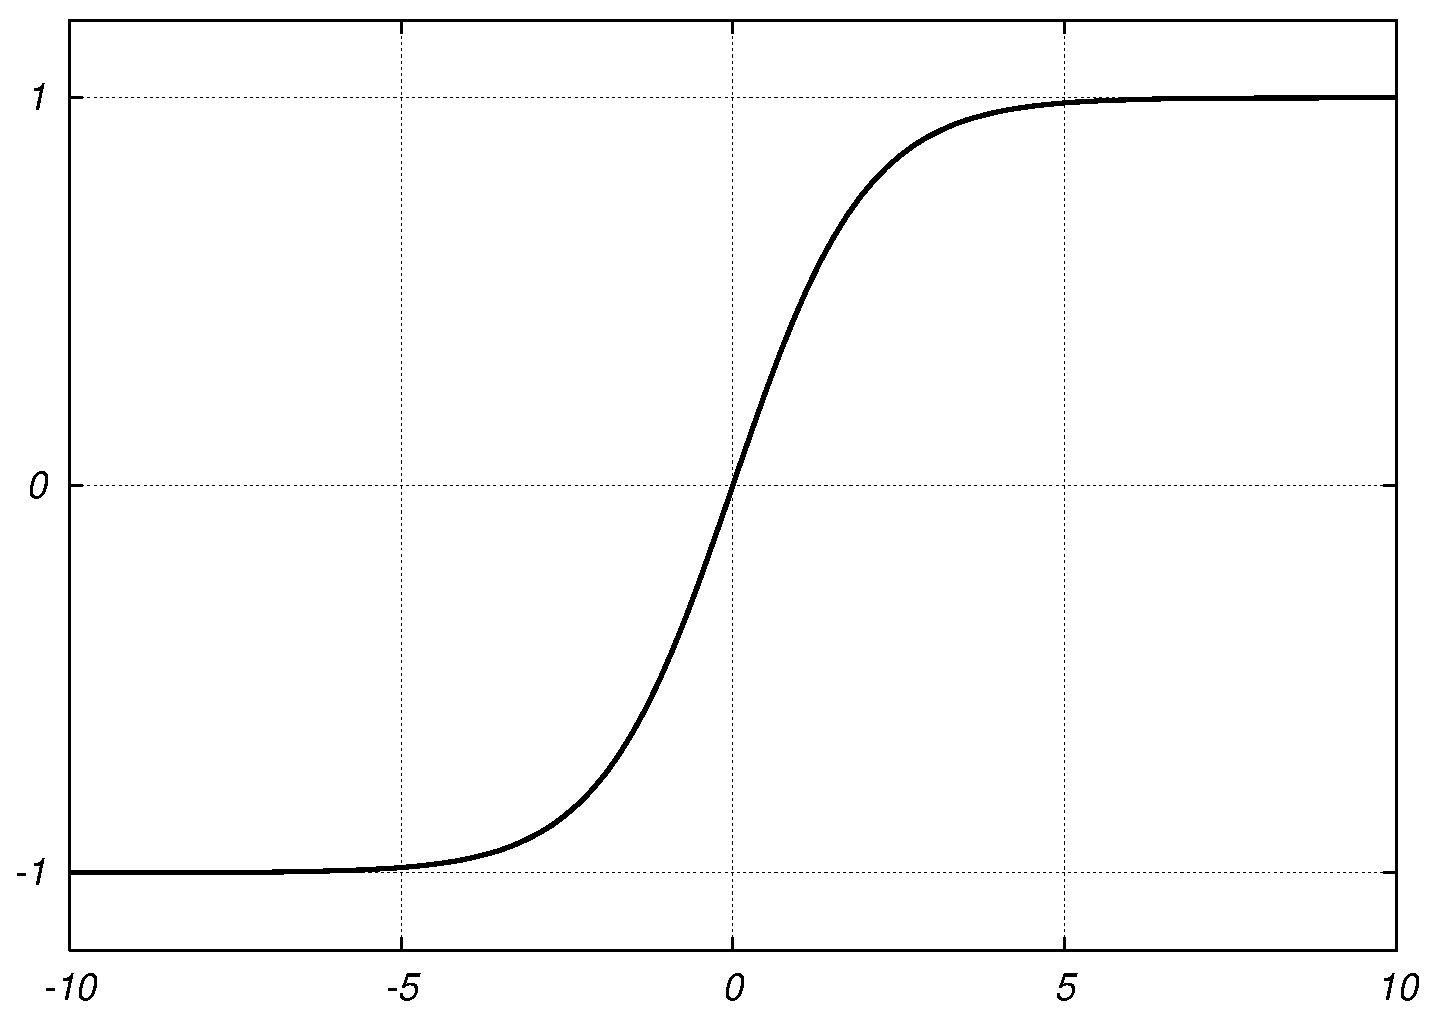
\includegraphics[width=0.45\textwidth,%
  totalheight=0.25\textheight]{tanh} &
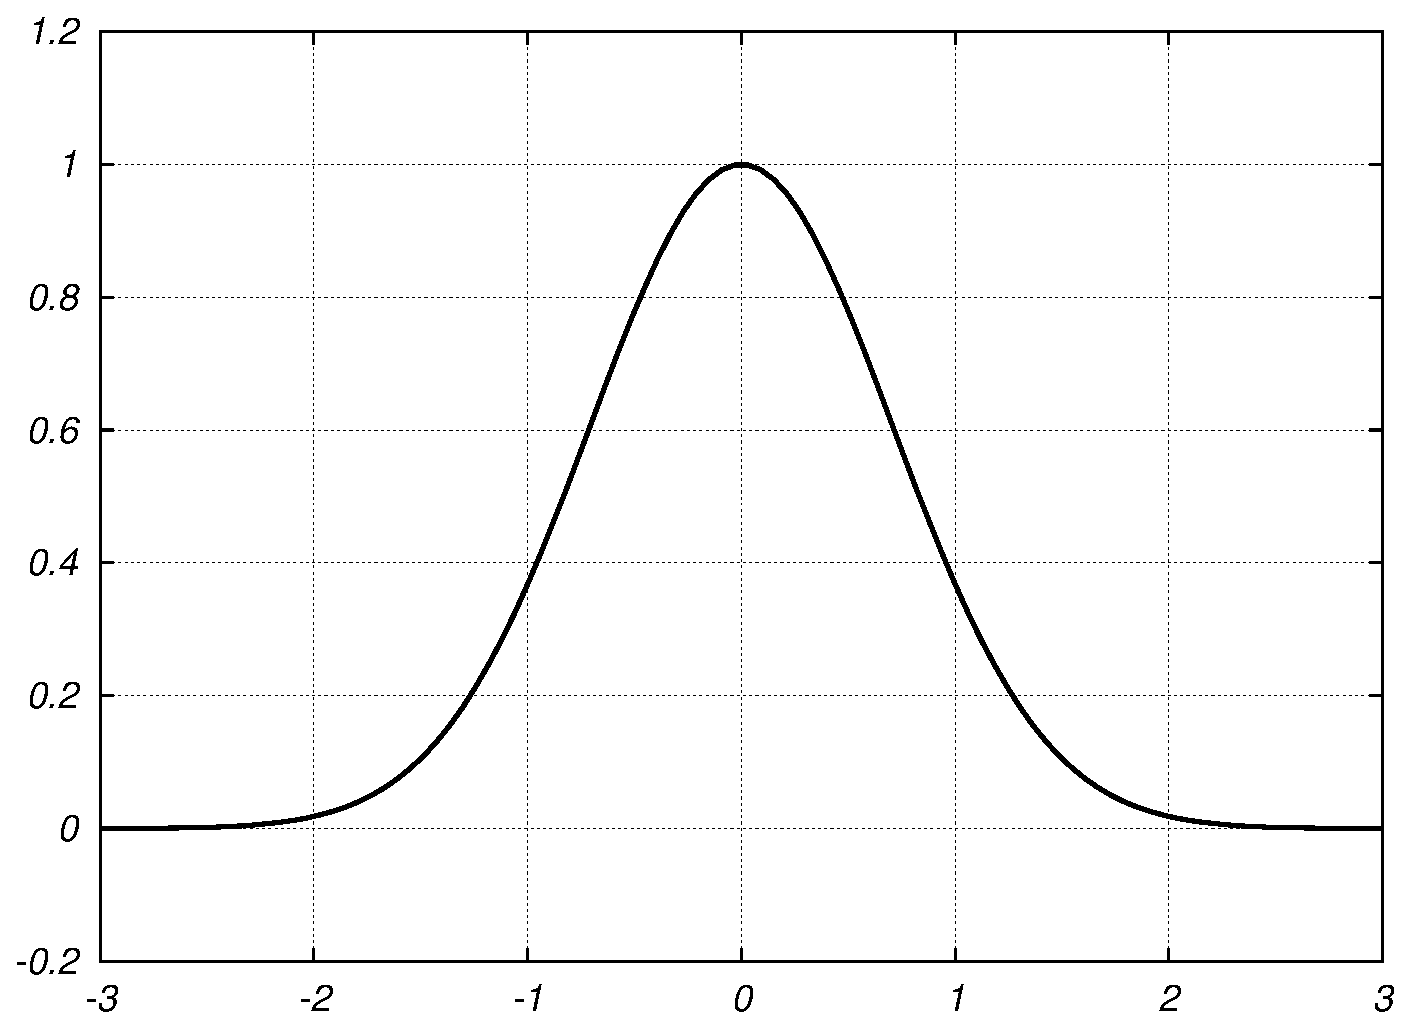
\includegraphics[width=0.45\textwidth,%
  totalheight=0.25\textheight]{rbf} \\
а) & б)\\
\end{tabular}
\caption{Функции $\fa$ сигмоидального (а) и радиально-базисного (б) типов.}
\label{fig:act_func}
\end{figure}

Рассмотрим типовую архитектуру многослойного персцептрона.  Нейроны в
сетях такого типа объединяются в сеть послойно.  За исключением
специальных случаев соединение нейронов в последовалельных слоях
полное, то есть, выход каждого нейрона $i$-го слоя подается на каждый
из нейронов $(i+1)$-го слоя.  Схема многослойной нейронной сети без
перекрестных и обратных связей приводится на \figref{fig:mlann}.

\begin{figure}[h]
\centering
% This does not make picture in PDF/LaTeX:
%\input{nn_arch.pic}
% So, let's do the next way:
% 1. xfig -specialtext -latexfonts -startlatexFont default nn_arch.fig
% 2. Update all text objects (with TeX special symbols) to Default font
% 3. Export to PS/LaTeX (changing default extension from .pstex to .eps)
% 4. Edit nn_arch.eps_t file and remove .eps extension from \includegraphics
% 5. Put next \input:
\input{nn_arch.eps_t}
\caption{Многослойная нейронная сеть прямого распространения.}
\label{fig:mlann}
\end{figure}

Для компактного описания архитектуры многослойной нейронной сети
удобно использовать обозначение $\NN_{n_0,n_1,\ldots,n_{m-1},n_m}$,
где $n_0$ --- число входов первого (входного) слоя сети,
$n_1,\ldots,n_{m-1}$ --- число нейронов в последовательно
расположенных скрытых слоях, $n_m$ --- число нейронов (и выходов)
последнего, выходного слоя.

\subsection{Выбор числа нейронов и архитектуры сети}

Оптимальный выбор количества нейронов и их распределения по слоям
является сложной проблемой.  В действительности, речь идет о числе
настраиваемых параметров --- весовых коэффициентов НС.  Известны
обоснованные методы выбора их числа для некоторых частных случаев, то
есть конкретных архитектур и прикладных задач (например, ассоциативная
память на основе НС с радиально-базисной функцией~\cite{koh80}).
Выбор количества нейронов в этом случае определяется количеством
распознаваемых образов.  В общем случае, НС с радиально-базисной
функцией требуют априорного задания не только количества нейронов, но
и координат центров.  Эти параметры наглядно интерпретируются как
количество и расположение узлов сетки, покрывающей входное
пространство НС.

Известна теорема \marginpar{Какая теорема?} о представительной
способности сети прямого распространения с архитектурой $\NN_{n,k,m}$
и сигмоидальной функцией активации~(\figref{fig:act_func}а).  Она дает
следующее граничное определению количества нейронов скрытого слоя при
решении задачи классификации $N$ образов обучающей выборки:

\begin{equation}\label{eq:neuron-number}
\displaystyle\frac{mN}{(n+m)(1+\log_2N)} \le k \le
m(N/n+1)+\displaystyle\frac{m}{n+m}(N/n+2)
\end{equation}

Теоретический анализ емкости нейронной сети с архитектурой
$\NN_{1,n,1}$ для задач классификации и интерполяции в общем виде
дается в \cite{sontag93}.  Там же отмечается, что выяснение
существования заданного числа весовых коэффициентов НС, реализующих
заданное отображение, в общем случае является NP-полной проблемой.

Однако, практика показывает, что в подавляющем большинстве случаев нет
необходимости в точном выяснении оптимального числа нейронов.
Приблизительная оценка как правило оказывается приемлемой.  Методы
оценки необходимого числа параметров носят эвристический характер и в
значительной степени опираются на априорные знания о предметной
области.

При распределении нейронов по слоям также применяют разнообразные
эвристики, базирующиеся на эмпирических фактах.  В частности,
известно, что трех- и четырехслойные сети демонстрируют более высокую
скорость сходимости, чем двухслойные с аналогичным числом весовых
коэффициентов.  В том случае, если отдельные слои НС решают выделенные
задачи, распределение нейронов по ним может рассматриваться независимо
(сети встречного распространения, когнитрон и неокогнитрон
Фукушимы~\cite{wasser92}).

Известны также подходы, заключающиеся в добавлении или удалении
нейронов для достижения их оптимального количества при решении
конкретной задачи~\cite{gibb96}.  Однако примеры применения этих
методов при решении задач управления автору неизвестны.  Очевидно,
потребность в этих методах возникает только в случае значительной
априорной неопределенности сложности задачи.

\subsection{Нейросетевые архитектуры с динамическими свойствами}

В нейронной сети прямого распространения вычисленные выходы однозначно
определяются по входам.  Для придания динамических свойств нейронным
сетям используются различные подходы:

\begin{itemize}

\item
параллельная подача на вход НС значений в последовательные моменты
времени (\figref{fig:dynamic_nn}а);

\item
локальные обратные связи в нейронах сети или ее специального
контекстного слоя: сети Элмана и Джордана~\cite{gibb96}\cite{golovko01};

\item
глобальные обратные связи в нейронной сети: сети Хопфилда и обратное
распространение ошибки во времени
(\figref{fig:dynamic_nn}б)~\cite{wasser92}\cite{golovko01}.

\end{itemize}

\begin{figure}[h]
\centering
\begin{tabular}{cc}
\hbox{\input{dnn_arma.eps_t}} &
\hbox{\input{dnn_feedback.eps_t}} \\
а) & б)\\
\end{tabular}
\caption{Способы придания динамических свойств нейронной сети с помощью
         разложения во временной ряд (а)
         и глобальной обратной связью (б).}
\label{fig:dynamic_nn}
\end{figure}

%В первых двух 

% Дополнительные комментарии на данную тему

\subsection{Алгоритмы обучения нейронных сетей}\label{nn_learning_algorithms}

Настройка нейронной сети на решение конкретной прикладной задачи
осуществляется путем однократной или итеративной процедуры задания
$w_j$ --- весовых коэффициентов нейронов.  В случае радиально-базисных
нейронов необходимо также задать $c_j$ --- центры функций.  В том
случае, если настройка НС ведется для решения задачи аппроксимации
некоторой неизвестной функции $f(.)$, заданной таблично, то такой
процесс называют обучением с учителем ({\em supervised learning}):
\begin{equation}\label{eq:supervised_learning_task}
  \begin{array}{c}
    \mathbf{y}_k=f(\mathbf{x}_k)\\
    \sum\limits_k\big(\mathbf{y}_k-\NN(\mathbf{x}_k)\big)^2\rightarrow\min
  \end{array}
\end{equation}

Классическим примером обучения с учителем является задача
аппроксимации функции ``Исключающее ИЛИ''.  Если же целевая функция не
задана явно, но имеются некоторые косвенные признаки ее достижения,
этот процесс называется обучением без учителя ({\em unsupervised
  learning}).  Таким, например, является решение задачи коммивояжера с
помощью нейронной сети Хопфилда~\cite{wasser92}.

При решении задач синтеза регуляторов целевая функция, которой обычно
является уставка, как правило, задана, поэтому наибольшее
распространение получили методы обучения с учителем.  Этот вид
обучения НС тесно связан с методами оптимизации, поэтому подходы и
проблемы обеих областей являются общими.  В частности, методы
оптимизации бывают градиентные и случайные.

Базовым градиентным методом обучения НС является обратное
распространение ошибки.  Он соответствует градиентному методу
оптимизации первого порядка, при котором для выбора направления
используется информация о первой производной функции ошибки.
Очевидные недостатки метода, связанные с линейностью процедуры поиска
минимума, устраняются в семействе методов второго порядка.  Среди них
есть как разработанные специально для обучения НС (QuickProp,
Delta-Bar-Delta и т. п.), так и имеющие важное значение в теории
оптимизации (методы сопряженных градиентов, Левенберга-Маркварта и
т. п.~\cite{himmelblau75}).  Исчерпывающий обзор градиентных методов
обучения НС и связанных с ними эвристик приводится в~\cite{gibb96}.

Следует различать принцип и метод обратного распространения ошибки.
Введем следующие обозначения для вычисления выхода сигмоидального
нейрона без порога:

\begin{equation}
\label{eq:sigm_neuron_output_parts}
\begin{array}{rcl}
  z^d_i & = & \sum\limits_j w^d_{ij}q^{d-1}_j \\
  q^d_i & = & \fa(z^d_i),
\end{array}
\end{equation} где $q^{d-1}_j$ и $q^d_i$ --- вход и выход $d$-го слоя
соответственно; $w^d_{ij}$ обозначает весовой коэффициент $j$-го входа
$i$-го нейрона слоя; $\fa(.)$ --- функция активации нейрона.
Отсутствие порога по сравнению с~\eqref{eq:sigm_neuron_output} не
снижает общности уравнения, так как можно считать, что некоторый вход
каждого нейрона всегда равен единице.  Коэффициент при этом входе
можно считать порогом.

Обобщенная ошибка $\delta$ распространяется через нейронную сеть в
обратном направлении (от выходов к входам) в соответствии с
уравнением, различающимся для выходного и скрытых слоев:

\begin{equation}
\label{eq:deltaprop}
  \delta^d_i=\left\{\begin{array}{ll}
    \fa'(z^d_i)\sum\limits_h\delta^{d+1}_h w^{d+1}_{hi} & 1\le d<m \\
    \fa'(z^d_i)(\hat{y}_{k+1}-r_{k+1}) & d=m \\
  \end{array}\right.
\end{equation}

Это уравнение определяет принцип обратного распространения и в нем нет
обучающей составляющей, так как весовые коэффициенты в нем неизменны.
Уравнение~\eqref{eq:deltaprop} справедливо для всех градиентных
методов обучения, в том числе для простейшего из них --- метода
обратного распространения ошибки.  В нем для обучения, то есть,
коррекции весовых коэффициентов, используется дельта-правило

\begin{equation}
\label{eq:weightchange}
  w^d_{ij}(k+1)=w^d_{ij}(k)-\eta\delta^d_i q^{d-1}_j
\end{equation} где $\eta$ --- коэффициент скорости обучения.

В других методах градиентного обучения используются более сложные
способы коррекции весового коэффициента, базирующиеся на адаптивном
коэффициенте скорости обучения (например, Delta-Bar-Delta) или
использующие информацию о коррекции весового коэффициента и обобщенной
ошибки с предыдущего шага (QuickProp).

Важным достоинством градиентных методов обучения является высокая
скорость сходимости, особенно присущая методам второго порядка.
Однако направленная процедура поиска может привести в локальный
минимум вместо глобального.  В общем случае проблема поиска
глобального минимума градиентным спуском не может быть решена.

Избежать градиентного спуска, а значит, попадания в локальные минимумы
возможно с помощью группы методов случайного поиска.  Один из них,
алгоритм {\it alopex}, упоминаемый в~\cite{boquete99}, основан на
корреляции ошибки и вариации весовых коэффициентов с использованием
полученной информации для их обновления в нужном направлении.  Следует
отметить также метод отжига, названный так по аналогии с физическим
процессом-прототипом~\cite{wasser92}.  Размер случайного шага в этом
методе регулируется ``температурой'' сети.  По мере понижения
температуры шаг статистически укорачивается, что в пределе локализует
зону поисков окрестностью глобального минимума.  К сожалению, в
простых ситуациях методы случайного поиска значительно медленнее
градиентных.  Кроме того, в процессе случайного поиска выход НС может
достаточно сильно отличаться от целевого значения.

Задачи синтеза нейросетевого регулятора и модели объекта управления с
точки зрения теории оптимизации являются, как правило, достаточно
простыми.  С другой стороны, потребность систем управления в адаптации
к изменяющимся условиям накладывает определенные требования к
быстродействию используемых алгоритмов обучения и предсказуемости
промежуточных результатов.  Эти соображения являются решающими при
выборе градиентых методов обучения НС, что подтверждается практикой их
повсеместного использования в системах автоматического управления.

%%%%%%%%%%%%%%%%%%%%%%%%%%%%%%%%%%%%%%%%%%%%%
\section{Особенности применения нейронных сетей в системах управления}

Анализ литературы показывает, что несмотря на многообразие примеров
применения нейронные сети могут выступать в системах управления всего
в нескольких разных ролях.  Каждая роль имеет свою специфику, что
накладывает определенные требования на архитектуру нейронной сети и
алгоритм ее обучения.  В большинстве из рассмотренных работ нейронная
сеть выступает в качестве:

\begin{enumerate}

\item
регулятора~\cite{sigom00}\cite{khomyu96}\cite{kav96}\cite{bouchard01}\cite{linwaihong01}\cite{gorfeld96}\cite{tukin01}\cite{pican95}\cite{golovko01}\cite{fabri98};

\item
модели объекта управления~\cite{narmuk96}\cite{park96}\cite{levinar95}\cite{kulee96};

\item
оптимального фильтра объекта управления~\cite{hayyeeder97};

\item
регулятора совместно с регулятором другого типа:
линейным~\cite{steck96}\cite{sigom00} \cite{chenmills97} и
нечетко-логическим~\cite{sigom00}\cite{wailinlin00}\cite{linwaihong01};

\item
настройщика регулятора другого типа~\cite{sigom00}\cite{samtar96};

\item
классификатора или распознавателя
образов~\cite{uhrig91}\cite{zhuchkov02}\cite{basubart94}\cite{golovko01}.

\end{enumerate}

В дальнейшем не будем рассматривать задачу классификации статических и
динамических образов, так как она является вспомогательной и выходит
за рамки собственно задач управления.  Сконцентрируем внимание на
особенностях реализации регуляторов с применением нейронных сетей, а
также сопряженными вопросами, в числе которых построение нейросетевой
модели объекта управления

\subsection{Нейросетевой регулятор}

%%%%%%%%%%%% Привести различные схемы включения по входам

% Управление по отклонению
Подобно традиционным регуляторам, нейросетевые регуляторы могут
подключаться как по возмущению, так и по отклонению.  В частности,
предлагаются варианты управления по отклонению, в которых нейронная
сеть регулятора имеет внешнюю архитектуру вида $\NN(e_k)$ (например,
в~\cite{ronco98}).
% Управление по возмущению
Архитектура нейросетевого регулятора $\NN(r_k)$, соответствующая
управлению по возмущению, применялась автором работы~\cite{khomyu96}.

% Совмещенное управление feedforward+feedback
Комбинированные схемы включения нейросетевого регулятора обычно имеют
архитектуру входов вида
$\NN(r_k,y_k)$~\cite{narpart92}\cite{trc95}\cite{samtar96}.  Учитывая
способность нейронных сетей к реализации разнообразных функций,
информационно этот вариант эквивалентен $\NN(e_k,y_k)$ и
$\NN(e_k,r_k)$, так как $e_k=r_k-y_k$.  Нейросетевой регулятор (НС--Р)
с архитектурой входов $\NN(e_k,y_k)$ предлагается в~\cite{narmuk96}.

Схема комбинированного нейросетевого управления приводится
в~\cite{sigom00}.  В работе~\cite{park96} подобная схема используется
для оптимального управления нелинейным динамическим объектом.  Одна из
нейронных сетей ($\NN^{FFC}$) является регулятором по возмущению, а
другая ($\NN^{FBC}$) использует информацию из обратной связи контура
управления и сама имеет обратную связь.  Управляющее воздействие на
объект вычисляется в соответствии с уравнением:

$$
u_{k}=\NN^{FFC}(r_k)+\NN^{FBC}(r_k, y_k, u_{k-1})
$$

\noindent
где $r_k$ --- уставка, $y_k$ --- наблюдаемый выход объекта управления,
$u_{k-1}$ --- управляющее воздействие, сформированное в предыдущий
момент времени.

% Другие схемы
В некоторых работах предлагаются НС--Р с производными различных
порядков от базовой величины на входе.  Очевидно, основное назначение
этих схем --- реализация динамических свойств в нейронной сети прямого
распространения.  Например, кроме уставки на вход нейросетевого
регулятора подаются дискретные производные первого и второго порядков:
$\NN(r_k,\dot{r}_k,\ddot{r}_k)$.  Есть примеры использования в
качестве входов производных сигнала ошибки:
$\NN(e_k,\dot{e}_k)$~\cite{wailinlin00}\cite{linwaihong01},
$\NN(e_k,\dot{e}_k,\ddot{e}_k,\ldots,{e}^{(n)}_k)$~\cite{eremin95}.  В
последней работе количество производных $n$ предлагается выбирать
исходя из порядка объекта.

Несмотря на обилие приводимых в литературе разнообразных способов
включения нейросетевого регулятора в контур управления остается
открытым вопрос о критериях выбора той или иной схемы и оптимальности
сделанного выбора для целевой задачи.  Ни в одной из рассмотренных
работ авторы не аргументируют выбор входов, опираясь на свойства
собственно нейронных сетей.  Как правило, выбор числа и номенклатуры
входов НС--Р осуществляется по аналогии с имеющимися регуляторами или
из экспертных соображений.

% Обучение
Рассмотрим предлагаемые в литературе основные способы настройки
нейросетевого регулятора.  Их достаточно полный сводный обзор
приводится в~\cite{sigom00}.  Отметим, что в общем случае способ
обучения не зависит от вида и количества входов НС--Р.

\subsubsection{Прямое инверсное регулирование}%
\label{direct_inv_nnc}

Случай включения НС--Р в качестве регулятора по возмущению приведен
на~\figref{fig:direct_nnc}б.  Сеть может настраиваться вне контура
управления по накопленным данным.  Для реализации динамических свойств
предлагается подавать параллельно на вход НС--Р задержанные во времени
наблюденные на выходе объекта значения~\figref{fig:direct_nnc}а.  В
процессе обучения нейронная сеть обучается прямой инверсии объекта
управления.  По окончании обучения НС--Р включается в контур
управления, но на ее вход подаются не наблюденные значения
$y_k,y_{k-1}$, а желаемые $r_k,r_{k-1}$.  Осуществляя инверсию
нейронная сеть генерирует такое управляющее воздействие $u_k$, чтобы
выход объект стал равным желаемому.

\begin{figure}[h]
\centering
\begin{tabular}{c}
\hbox{\input{nnc_direct_inv_tr.eps_t}} \\
а) \\
\hbox{\input{nnc_direct_inv_ev.eps_t}} \\
б)\\
\end{tabular}
\caption{Прямое инверсное регулирование: схема обучения (а)
         и рабочего функционирования (б).}
\label{fig:direct_nnc}
\end{figure}

Основным недостатком приведенной схемы является необходимость в том,
чтобы объект управления был обратимым.  Это не всегда имеет место.
Кроме того, задача построения инверсии функции требует достаточно
плотного покрытия области аргументов и области значений
экспериментальными точками, используемыми для обучения НС--Р.  Объем
этого множества полиномиально растет с увеличением размерности входов
и выходов, что делает обучение нейронной сети очень длительной
процедурой.  Снижение плотности покрытия приводит к плохому качеству
инверсии.

\subsubsection{Специализированное обучение}

Другая схема обучения НС--Р, приведенная на~\figref{fig:special_nnc},
предполагает подстройку весовых коэффициентов нейронной сети в
процессе ее рабочего функционирования.  Градиентный алгоритм обучения
НС--Р использует информацию об ошибке управления и активируется каждый
такт времени.  Для приведения ошибки к выходу нейросетевого регулятора
необходимо знать мгновенное значение якобиана объекта управления.  Это
не всегда возможно, поэтому часто довольствуются знаком якобиана,
показывающим направление, в котором надо изменять управляющее
воздействие для уменьшения ошибки управления.

\begin{figure}[h]
\centering
\input{nnc_special_tr.eps_t}
\caption{Схема специализированного обучения.}
\label{fig:special_nnc}
\end{figure}

Очевидным недостатком описанного подхода является неопределенность
выхода нейронной сети в первый момент обучения.  Поскольку
одновременно с обучением НС--Р управляет объектом, по сути случайное
значение $u_0$ может привести в реальной системе управления к
катастрофическим последствиям.  Несмотря на то, что данная особенность
в литературе не подчеркивается, очевидно, что специализированное
обучение в чистом виде не применимо на практике.

\subsubsection{Косвенное адаптивное регулирование}

Как уже отмечалось, оценка мгновенного значения якобиана объекта
управления представляет определенные трудности.  Суть этих трудностей,
а также способ оценки якобиана с помощью нейронной сети излагается в
п.~\ref{identif_and_nnp}.  Вариант обучения НС--Р с использованием
нейросетевой оценки якобиана~(\figref{fig:indirect_nnc}) в разных
работах называется по-разному: косвенным адаптивным
управлением~\cite{narpart92}, обратным распространением во времени
(Вербос), обучением с нейроэмулятором~\cite{sigom00}.  Множественность
названий проистекает из того, что основы нейросетевой версии метода
были опубликованы независимо в двух работах, кроме того принципиальная
схема была до этого известна в традиционной теории управления.

\begin{figure}[h]
\centering
\input{nnc_indirect_inv_tr.eps_t}
\caption{Схема косвенного адаптивного нейросетевого регулирования.}
\label{fig:indirect_nnc}
\end{figure}

В главном данный метод аналогичен специализированному обучению за
исключением способа оценки якобиана.  Однако именно использование
нейросетевого эмулятора делает косвенное адаптивное управление
чрезвычайно ценным и популярным подходом.  Нейросетевая модель объекта
управления (НС--О) позволяет на такте обратного распространения ошибки
оценить якобиан достаточно точно, что позволяет при соблюдении
определенных требований к параметрам градиентного алгоритма обучать
НС--Р и НС--О одновременно.  Очевидно, что подстройка обеих нейронных
сетей позволяет адаптировать систему управления к изменению параметров
объекта и внешних условий.

Отметим, что оценивание якобиана объекта управления является косвенным
методом инверсии объекта, отличающимся от прямого, рассмотренного в
п.~\ref{direct_inv_nnc}.  В отличие от прямой инверсии косвенная
реализуется алгоритмом обратного распространения ошибки.

%  В отличие от прямой инверсии обратимость
%объекта управления не является существенной, так как на такте
%обратного распространения ошибки управления через НС--О производится
%мгновенная оценка якобиана, локальная в точке, описывающей текущее
%состояние объекта.

Часто рассматриваемая схема ассоциируется с одним из методов обучения
нейронных сетей с обратными связями --- обратным распространением во
времени ({\it backpropagation through time --- BPTT}).  Однако, при
использовании архитектур НС без обратных связей возможно применение
косвенного адаптивного управления вместе с другими, более простыми,
чем BPTT, методами обучения нейронных сетей~\cite{narpart92}.

В работе~\cite{fabri98} предлагается оригинальный метод оперативного
обучения нейросетевого регулятора, основанный на калмановском
оценивании значений параметров.  При этом подразумевается, что
нейросетевая модель объекта в заданном диапазоне аппроксимации
функционирует точно.  Метод предназначен для нейросетевого
регулирования нелинейным объектом, афинным по управлению, с аддитивной
помехой в канале наблюдения.  Преимуществом изложенного метода по
сравнению с другими схемами является учет неопределенности состояния
объекта в первые моменты времени работы САУ.  Рассматриваются решения,
основанные как на многослойном перцептроне, так и на сети нейронов с
радиально-базисной функцией.

%\subsection{Нейросетевая модель объекта управления}

%В простейшем случае при решении задачи синтеза нейросетевого аналога
%имеющегося регулятора желаемый выход для любого входного значения
%может быть легко получен.  Пары ``вход--выход'', накопленные за время
%наблюдения за исходной системой автоматического управления можно
%использовать в дальнейшем при настройке нейронной сети вне контура
%подобно регулятору-прототипу.

\subsection{Идентификация и нейросетевая модель объекта управления}%
\label{identif_and_nnp}

При синтезе нейросетевого регулятора, реализующего некоторый новый
закон управления, возникает вопрос с формированием желаемого выхода
регулятора по заданному входу.  Из теории управления известно, что
сформировать идеальное управляющее воздействие на объект можно зная
мгновенное значение якобиана --- матрицы частных производных вектора
состояния объекта управления по переменным управляющего воздействия.
Целью этой операции является перевод объекта управления из текущего
состояния в желаемое.

В моделируемой ситуации якобиан легко расчитывается аналитически по
модели объекта и его значение может использоваться при настройке
нейронной сети регулятора.  Однако для большинства реальных объектов
управления модель приходится получать или уточнять с помощью методов
идентификации.

Классический метод идентификации линейных систем управления
основывается на качественном определении структуры объекта по
переходной характеристике и на частотном анализе, применяемом для
уточнения параметров объекта.  Данный подход с трудом поддается
автоматизации, поскольку базируется на экспертных знаниях инженера.

Одним из наиболее эффективных и удобных для реализации на современных
компьютерах методов идентификации неизвестных параметров многомерных
систем является алгоритм Качмажа~\cite{bolonchin91}.  Он позволяет
итерационно определить матрицу $A$ неизвестных параметров линейной
дискретной системы вида:

\begin{equation}\label{kachmaj}
\mathbf{x}_k=A^T \mathbf{u}_k
\end{equation} где $\mathbf{u}_k$ --- управляющее воздействие, а
$\mathbf{x}_k$ --- наблюдаемое состояние объекта управления.

Другой метод идентификации изложен в~\cite{boxjenk74}.  Он состоит из
двух этапов, на первом из которых принимается решение о виде модели
объекта, а на втором уточняются параметры модели и оценивается ее
статистическая достоверность.  Модель строится в форме линейного
разностного уравнения:

\begin{equation}\label{arima}
x_k=\delta^{-1}(B)\omega(B) u_{k-b} + n_k
\end{equation} где $B=1-\nabla$ --- оператор сдвига назад, $n_k$ ---
случайная помеха, описываемая процессом АРСС, $\delta$ и $\omega$ ---
полиномы.

Перечисленные методы существенно связаны с гипотезой о линейности
исследуемого объекта управления и по этой причине плохо подходят для
идентификации нелинейных объектов, особенно в том случае, если вид
нелинейности априорно неизвестен.  С другой стороны, нейросетевой
регулятор реализует существенно нелинейную функцию, поэтому его
применение весьма целесообразно для как можно более широкого класса
объектов управления.  По этой причине предложенные выше методы
построения модели объекта при формальной возможности их использования
для оценки якобиана значительно ограничивают область применения
нейросетевого регулирование, снижая его ценность как метода решения
сложных задач управления.

%%%%%%%%%

Рассмотрим нейросетевую идентификацию, как альтернативу традиционным
методам и как наиболее подходящий метод оценки якобиана при синтезе
нейросетевых регуляторов.  Для простоты рассмотрим объект управления,
описываемый моделью SISO ({\it single input, single output} --- один
вход и один выход).  В дискретном времени в терминах пространства
состояний объект управления можно представить следующей системой
разностных уравнений:

\begin{equation}\label{eq:siso}
\left\{\begin{array}{rcl}
  \mathbf{x}_{k+1} & = & f(\mathbf{x}_k, u_k) \\
  y_k & = & g(\mathbf{x}_k)
\end{array}\right.
\end{equation} где $y_k$ и $u_k$ --- скаляры, а $\mathbf{x}_k$ --- вектор
состояния объекта в дискретный момент времени $k$.

Нейронная сеть прямого распространения, реализующая функцию
$\hat{y}_{k+1} = \NN^o(u_k)$, принципиально не может решить задачу
имитации поведения динамического объекта \eqref{eq:siso}, так как
нейросеть не обладает памятью: в любой момент выход нейронной сети
прямого распространения полностью определяется её актуальными
входами и не зависит от состояния нейросети в предыдущие моменты
времени, а также от прошлых входов.

Для построения адекватной динамической модели следует снабдить
нейросеть информацией о прошлых состояниях.  В литературе по
нейросетевому управлению известно несколько способов решения этой
проблемы.  Наиболее очевидный из них предполагает использование
обратных связей внутри нейронной сети для сохранения состояния между
рабочими тактами.  Второй состоит в добавлении внешних обратных связей
к базовой нейросети прямого распространения.  Третий вариант
предполагает непосредственное повторение нескольких прошлых наблюдений
с целью ``напомнить'' нейросети о состоянии моделируемого объекта в
предыдущие моменты времени.  Четвертым вариантом является подход,
объединяющий два предыдущих.  Рассмотрим их подробнее.

\subsubsection{Внутрение обратные связи}

Один из возможных вариантов модели с внутренним состоянием нейронной
сети предложен в~\cite{boquete99}.  Архитектура описанной нейросетевой
модели представляет собой расширенный вариант радиально-базисной сети
с FIR фильтром в локальной обратной связи.  Функционирование нейрона в
нейросетевой модели описывается
уравнением~\eqref{eq:rbf_neuron_output}, однако радиально-базисная
функция $R(.)$ вычисляется по более сложной формуле, включающей
локальные обратные связи:

$$
R_j\bigl(\mathbf{x}(k)\bigr)=
   \exp\Bigl[-\frac{1}{\sigma^2}\sum\limits_{i=1}^M
             (x_i(k)+\tilde{x}_{ji}(k)-c_{ji})^2\Bigr]
$$

$$
\tilde{x}_{ji}(k)=\sum\limits_{s=1}^S a_{jis}R_j\bigl(\mathbf{x}(k-s)\bigr)
$$

Настройка такой нейронной сети проводится с помощью адаптированного
градиентного метода и имеет целью коррекцию весовых коэффициентов
нейронной сети $w_i$ и FIR фильтра $a_{jis}$.  В
работе~\cite{boquete99} не предложено аргументированного способа
выбора глубины обратной связи $S$.

Другой вариант нейросетевой модели, предложенный в~\cite{benne00}
имеет архитектуру сети Элмана~\cite{golovko01}.  Нейронная сеть имеет
внешнюю архитектуру
$\hat{y}_{k+1}=\NN^o(x_{k-1-n_L},\ldots,x_{k-n_b-n_L})$, где $n_b$ ---
априорно заданный параметр регрессии, $n_L$ --- априорно заданный
параметр запаздывания.  Контекстный слой состоит из $n_a$ значений
$\hat{y}_{k},\ldots,\hat{y}_{k-n_a+1}$.  Параметры архитектуры
нейросетевой модели $n_a$, $n_b$, $n_L$ определяются экспертом на
основании априорных знаний об объекте.

\subsubsection{Внешние обратные связи}

Нейросетевая модель объекта в рамках данного подхода оснащается
дополнительным входом, на который подается выход модели,
полученный в предыдущий момент времени~\cite{sigom00}:
$$ \hat{y}_{k+1}=\NN^o(u_k, \hat{y}_k) $$

Задержанный сигнал обратной связи $\hat{y}_k$ имеет смысл памяти
состояния.  Схема модели приводится на~\figref{fig:nnp-feedback}.

\begin{figure}[h]
  \centering
  \input{nnp_feedback.eps_t}
  \caption{Модель с внешней обратной связью.}
  \label{fig:nnp-feedback}
\end{figure}

Для обучения нейронных сетей с внешними обратными связями можно
использовать метод обратного распространения в
времени~\cite{gibb96}\cite{sigom00}.

Применительно к рассматриваемой задаче данный подход имеет то
преимущество, что для обучения НС--О требуется только выборка
обучающих пар $(u_k, y_k)$, записанных при управлении объектом в
замкнутом контуре.  Сам объект при обучении и при функционировании
модели не используется.  Это означает, что время и методы настройки
(проверки) модели ничем не ограничены.  Нейросетевая модель объекта в
данном случае является полностью автономной.  Она имитирует {\it
поведение }объекта.  Поэтому обучение нейросетевого регулятора по
нейросетевой модели поведения возможно вне контура управления.

Однако в литературе отмечаются и недостатки BPTT.  Алгоритм обучения
является очень тяжелой в вычислительном отношении процедурой, требует
много памяти для сохранения полного состояния сети на протяжении
длительного времени для последующей обработки в обратном
направлении~\cite{levinar95}.  Кроме того, обнаружено, что нейросеть с
внешними обратными связями выявляет короткие зависимости в обучающей
последовательности, но не может научиться длинным в силу многократного
ослабления информации о зависимости в обратной связи в процессе
обратного распространения ошибки~\cite{linetal}.  Это свойство названо
эффектом исчезающего градиента ({\em vanishing gradient}).

Применительно к задаче нейросетевой имитации объекта управления
проблема исчезающего градиента возникает в двух случаях:
\begin{itemize}\label{simple-feedback-defects}
  \item значительное чистое запаздывание в динамике объекта
  управления;
  \item шаг квантования времени слишком мал по сравнению с
  характерным временем наступления установившегося режима.
\end{itemize}

\subsubsection{Повторение прошлых состояний}

Обратной связи вокруг НС--О можно избежать, если использовать для
нейросетевого моделирования динамики объекта несколько прошлых его
состояний, которые непосредственно наблюдались в предыдущие моменты
времени.  В этом случае прогноз выхода объекта нейросетью каждый раз
строится только на основе реальной информации из контура управления:

\begin{equation}\label{eq:past-states}
  \hat{y}_{k+1}=\NN^o(u_k, u_{k-1},\ldots,u_{k-D_u}, y_k,
                           y_{k-1},\ldots, y_{k-D_y})
\end{equation}

Данный подход применяется во многих работах, например
в~\cite{kulee96}\cite{levinar95}.  Схема одной из возможных моделей с
повторением прошлых состояний приводится
на~\figref{fig:nnp-past-states}.

\begin{figure}[h]
  \centering
  \input{nnp_paststates.eps_t}
  \caption{Пример модели с повторением прошлых состояний
  $\hat{y}_{k+1}=\NN^o(u_k, y_k, y_{k-1})$.}
  \label{fig:nnp-past-states}
\end{figure}

Обучение этой модели осуществляется вне контура управления на
некоторой тестовой выборке, включающей временные ряды $u_k$ и $y_k$.
Нейронная сеть $\NN^o$ обучается делать прогноз состояния
объекта максимально близко к реально наблюдавшемуся значению.
Поскольку в данной схеме обратная связь отсутствует, возможно
использование любого из методов обучения статических нейронных сетей,
например, стандартного метода обратного распространения.

После сеанса обучения настроенная нейросеть может использоваться в
контуре управления для предсказания выхода объекта и для настройки
нейрорегулятора.  Такая модель не является автономной.  Она опирается
на информацию об истинном, а не предсказанном на предыдущих шагах
состоянии объекта.  Иными словами, это модель {\it предсказания
}выхода объекта управления.

Модель повторения прошлых состояний может использоваться для инверсии
объекта управления, однако вследствие неавтономности модели необходимо
использовать наблюдаемые состояния объекта управления для его
инвертирования и, значит, для обучения нейрорегулятора.  Иными
словами, обучение нейросетевого регулятора должно осуществляться в
контуре управления в режиме рабочего функционирования.

\subsubsection{Гибридная модель}

Следует отметить, что возможно объединение обеих моделей в рамках
единого гибридного подхода, схема которого представлена
на~\figref{fig:nnp-hybrid}~\cite{park96}.  То есть, в модели
реализуется функция:

\begin{equation}\label{eq:nnp-hybrid}
  \hat{y}_{k+1}=\NN^o(u_k, u_{k-1},\ldots,u_{k-D_u}, \hat{y}_k,
                              \hat{y}_{k-1},\ldots, \hat{y}_{k-D_y})
\end{equation}

\begin{figure}[h]
  \centering
  \input{nnp_hybrid.eps_t}
  \caption{Пример гибридной модели
  $\hat{y}_{k+1}=\NN^o(u_k, \hat{y}_k, \hat{y}_{k-1})$.}
  \label{fig:nnp-hybrid}
\end{figure}

Для обучения нейросети необходимо использовать усложненный алгоритм
обратного распространения во времени, учитывающий задержки.

В данной модели ослаблено влияние недостатков модели с внешними
обратными связями (см. \pgref{simple-feedback-defects}).  В частности,
задержанные на величину чистого запаздывания входы регулирующего
воздействия должны помочь преодолеть первый недостаток, а обратная
связь с повторением нескольких задержанных выходов НС--О --- второй.

По сравнению с моделью повторения прошлых состояний объекта управления
гибридная модель, во-первых, является автономной, во-{вто-рых}, нейросеть
становится более гибкой в части обучения динамике объекта.

Однако необходимо упомянуть также еще один существенный практический
недостаток моделей с внешними обратными связями (в том числе и
гибридной).  Это медленная скорость обучения нейросети, на порядки
уступающая скорости обучения нейросети без обратных связей.

\subsubsection{Множественные модели}

В работах~\cite{narmuk96}\cite{ronco98} предлагается использовать
несколько моделей одновременно, выбирая в каждый момент времени ту из
них, которая дает наилучшее приближение фактического выхода объекта
управления.  В работе~\cite{ronco98} для выбора модели используется
радиально-базисная нейронная сеть.  Это позволяет лучше обрабатывать
ситуации, когда объект оказывается в точке бифуркации.

Подключение множественных моделей не предполагает наложение каких-либо
условий на их архитектуру.  В частности, это могут быть как
традиционные, так и нейросетевые модели.

\subsubsection{Улучшенное оценивание якобиана}

Традиционная квадратичная функция стоимости $E=\frac{1}{2}(\hat{y}_k -
y_k)^2$, используемая при настройке нейросетевой модели объекта вне
контура управления, требует достаточно больших экспериментальных
выборок для получения адекватной модели.  При оперативном дообучении
модель должна подстраиваться к изменившимся свойствам объекта гораздо
быстрее.  В работе~\cite{wangbao00} при оперативной подстройке SISO
модели объекта предлагается использовать модифицированную функцию
стоимости, включающую непосредственно ошибку оценки якобиана:

$$
E=\frac{1}{2}\Bigl\{\bigl(\hat{y}_k - y_k\bigr)^2 +
  \lambda\bigl(\frac{\partial\hat{y}_k}{\partial u_{k-1}} -
  J^B_k\bigr)^2\Bigr\}
$$

\noindent где $J^B_k$ --- действительный якобиан объекта, принудительно
ограниченный $-J^B\le J^B_k\le J^B$, а $\lambda$ --- весовой
коэффициент, который, как показывается в статье, должен быть меньше
единицы.  Приводятся граничные оценки коэффициентов скорости обучения
НС--О и НС--Р, гарантирующие устойчивость процесса одновременной
настройки нейронных сетей.  Аналитические расчеты иллюстрируются
результатам имитационных экспериментов, проводимых на нелинейных
объектах с гауссовской помехой.

%%%%%%%%%

\subsection{Совместное использование регуляторов различных типов}

Нейронные сети часто используются в системах управления параллельно
или последовательно с регуляторами других типов, обычно линейными ПИД
регуляторам~\cite{steck96}\cite{sigom00}\cite{chenmills97}.

Среди причин совмещения традиционных промышленных регуляторов с
нейросетевыми называют:

\begin{itemize}

\item
необходимость компенсации с помощью НС--Р нелинейных эффектов,
неустранимых при традиционном регулировании;

\item
адаптация контура управления к медленному изменению свойств объекта
или среды путем дообучения НС--Р;

\item
стабилизация контура с НС--Р посредством внешнего контура с ПИД
регулятором;

\item
устранение с помощью линейного регулятора эффекта перманентной
ненулевой ошибки, часто возникающей при чисто нейросетевом
регулировании.

\end{itemize}

Очевидно, что совмещение линейных и нейросетевых регуляторов является
попыткой устранения недостатков обоих подходов.  Насущной задачей с
этой позиции является выявление отличий нейросетевых регуляторов по
сравнению с традиционными.  В некоторых работах (например,
\cite{chenmills97}) отмечаются некоторые неочевидные свойства
нейросетевых регуляторов.  В работе~\cite{warwick96} нейронные сети
критикуются с позиций ортодоксальной неадаптивной линейной теории
управления, что представляется спорным по самой постановке вопроса.
% бухгалтерская точность при макроэкономических выкладках
Работа~\cite{khomyu96} содержит результаты сравнения регуляторов
нескольких типов, однако опубликованные результаты имеют интегральный
характер, не позволяющий оценить применимость каждого из регуляторов в
узкой прикладной области.  Вместе с тем, ни в одной из доступных
автору работ не проводится систематического сравнительного
исследования, позволяющего сопоставить свойства традиционных линейных
и нейросетевых регуляторов в деталях.  Актуальность такого
исследования не вызывает сомнений, так как позволит снизить как
имеющийся скепсис, так и необоснованный энтузиазм исследователей и
инженеров.

Кроме того, в литературе встречаются примеры совмещения свойств
нечетко-{логичес\-ких} регуляторов и нейронных
сетей~\cite{sigom00}\cite{linwaihong01}.

Объединение обычно осуществяется на основе радиально-базисных сетей.
Функция активации в этих сетях имеет форму, часто используемую для
определения нечектой принадлежности.  Выбор координат центров
радиально-базисных функций нейронов также можно рассматривать с точки
зрения нечетко-логического подхода.  Методы обучения таких регуляторов
традиционно нейросетевые, в частности используется парадигма
косвенного адаптивного управления~\cite{wailinlin00}.  В этой работе
нечетко-лигический нейросетевой регулятор включен параллельно с ПИД
регулятором, что позволяет гарантировать устойчивость контура
одновременно с устранением нелинейного трения, имеющегося в
рассматриваемой системе управления.

\subsection{Оптимальная нейросетевая фильтрация}

Наличие помех значительно усложняет задачу управления объектом.  В
простейшем случае известного линейного стационарного объекта и таких
же сигналов выделение достоверных данных возможно с помощью
Винеровской фильтрации.  В нестационарном линейном и многих нелинейных
случаях задача наблюдения успешно решается с помощью фильтра Калмана.
Тем не менее, есть ситуации, в которых применение калмановской
фильтрации неэффективно.

Нейросетевой подход к оптимальной нелинейной фильтрации излагается
в~\cite{hayyeeder97}.  Авторы анализируют ключевые работы в данной
области и предлагают фильтр на основе нейронной сети с
радиально-базисными функциями.  В работе приводятся результаты
успешного применения предложенного фильтра в существенно нелинейных
случаях.  Опубликованы также данные сравнительных экспериментов с
другим нейросетевым фильтром, предложенным ранее и основанным на
многослойном перцептроне с обратными связями.


\subsection{Нейронная сеть в качестве настройщика регулятора}

В некоторых работах предлагается использовать адаптивные свойства
нейронных сетей не напрямую, а опосредованно, для настройки регулятора
другого типа.  Например, в~\cite{samtar96} рассматриваются два
варианта подбора параметров ПИД регулятора с использованием нейронной
сети.  Первый подход представляет собой схему косвенного адаптивного
управления с автономной нейросетевой моделью объекта, используемой для
настройки ПИД регулятора.  Идея второго подхода заключается в том,
чтобы напрямую использовать выходы НС для получения требуемых
параметров настраиваемого регулятора: $K_P$, $K_I$, $K_D$
(см.~\figref{fig:nn-tunes-pid}).

\begin{figure}[h]
  \centering
  \input{nn_tunes_pid.eps_t}
  \caption{Настройка ПИД регулятора с помощью нейронной сети.}
  \label{fig:nn-tunes-pid}
\end{figure}

В \cite{sigom00} приводится похожая схема настройки ПИД регулятора,
однако в качестве входов НС предлагается использовать тройку $r_k$,
$u_{k-1}$, $y_k$.  Критерием оптимизации выступает традиционная
квадратичная функция стоимости $E=\frac{1}{2}(r_k^2-y_k^2)$.

Предложенный подход представляет значительный практический интерес в
случае строго линейного объекта управления.  Использование ПИД
регулятора упрощает анализ устойчивости, однако для нелинейных
объектов во многих случаях нейросетевой регулятор будет более
эффективным.


\section{Проблема сопоставления нейросетевых и линейных регуляторов}

Современные промышленные системы управления в большинстве своем
основаны на подходах линейной теории автоматического
регулирования~\cite{warwick96}.  Это касается как моделей объектов,
рассматриваемых в линейном приближении, так и регуляторов, в
большинстве своем, ПИД (в Японии, например, доля ПИД регуляторов
составляет 84\%~\cite{sigom00}).  Соответственно, применение
нейросетевого управления в промышленности объективно требует
сопоставления с другими подходами, прежде всего, традиционным ПИД
управлением.  Это тем более важно, что НС является существенно
нелинейным объектом и включение ее в контур управления меняет свойства
всей системы.

В работе~\cite{khomyu96} приводятся результаты сопоставления
нечетко-логического, {нейросете\-во\-го}, ПИ и линейного адаптивного
регулятора ({\em general predictive controller}).  Сравнение
осуществляется на примере управления температурой в бассейне.  Оценке
подвергается как методика синтеза регулятора (потребность в модели
объекта управления, возможность самонастройки, вычислительная
сложность используемых алгоритмов), так и результат управления в
различных ситуациях (номинальные условия, пиковые помехи, изменение
времени задержки объекта управления и других его параметров).
Отдельно оцениваются точность управления и плавность выдаваемых
управляющих воздействий.  Оценки, приводимые в результирующей таблице,
носят лингвистический характер (``плохо'', ``средне'', ``хорошо'',
``лучше всех''), что позволяет инженеру сделать выбор метода
регулирования при проектировании схожей САУ.  Однако отсутствует
информация о собственно свойствах нейронных сетей в контексте
сравнения с другими регуляторами.  Авторы публикации не дают
детального анализа причин позиционирования рассматриваемых регуляторов
по выбранным критериям, в то время как даже методика подобного анализа
позволила бы значительно повысить ценность работы при проектировании и
анализе САУ других типов.  В другой работе тех же
авторов~\cite{sigom00} также не приводятся более подробные сведения о
проведенных экспериментах, констатируется лишь факт улучшения качества
управления по сравнению с линейным случаем.

В работе~\cite{boquete99} приводятся графики ошибки линейной и угловой
скорости в случаях ПИД регулирования и совмещенного ПИД--НС
регулирования.  Отмечается, что применение НС позволило уменьшить
перерегулирование в начальный момент времени, что способствовало
большей плавности хода.  Однако точные числовые оценки качества
управления в статье не приводятся.

Другой случай сопоставления линейного и нейросетевого гибридного
регуляторов на задаче управления сервомотором приводится
в~\cite{wailinlin00}.  Авторы отмечают, объект управления эффективно
линеаризуется, однако в процессе эксплуатации имеют место возмущения,
привносимые нагрузкой сервомотора, существенно ухудшающие качество
управления с ПИ регулятором в контуре.  Адаптивный гибридный
нейросетевой--не\-чет\-ко\-ло\-ги\-че\-ский регулятор, используя информацию о
якобиане объекта управления с нейросетевой модели, помогает уменьшить
перерегулирование в при ступенчатой нагрузке в 3 раза по сравнению с
ПИ вариантом.  Синтез ПИ регулятора проводился с целью оптимизации
параметров переходного процесса во временной области, а нейросетевой
регулятор и модель настраивались по критерию минимизации
среднеквадратичной ошибки.

Часто в работах по нейросетевому регулированию сравнение с
традиционными регуляторами имеет демонстрационный характер, при этом
подчеркивается факт улучшение качества регулирования на приведенных
примерах.  Отсутствуют эксперименты, демонстрирующие преимущества
линейных регуляторов перед нейросетевыми с подробным анализом
результатов.  Очевидно, такие примеры должны быть, однако их
отсутствие в литературе свидельствует о неполноте знаний по применению
НС в системах управления.

Попытки целенаправленного и рационального осмысления места нейронных
сетей в линейных системах предпринимаются в работах~\cite{warwick96}
и~\cite{toudeft}.  В первой из них справедливо отмечается, что
корректным линейным прототипом для нейросетевого регулятора является
дискретный оптимальный регулятор.  Далее автор упрощает многослойный
персептрон, заменяя нелинейную функцию активации линейной и, сравнивая
количество параметров с линейными системами АРСС, приходит к выводу о
неэффективной параметризации линейных систем с помощью нейронных
сетей.  Как следствие, избыточное число параметров приводит к
замедлению сходимости в процессе обучения и неточности оценки истиных
значений параметров.  Результаты работы не имеют той ценности, какую
могли бы иметь, если бы рассматривались нелинейные НС, для которых
имеются многочисленные примеры их успешного использования при имитации
линейных объектов и управления ими
(например,~\cite{khomyu96}\cite{wailinlin00}\cite{elfil-pta99}).

Во второй работе~\cite{toudeft} настройка НС--Р осуществляется по
схеме косвенного адаптивного управления линейным неустойчивым объектом
с чистым запаздыванием.  При синтезе НС--О порядок объекта считается
известным, а оценка запаздывания производится традиционным анализом
отклика на ступенчатое возмущение.  Особенность данной работы в том,
что нейронные сети НС--О и НС--Р редуцированы до одного нейрона с
линейным выходом.  Подобная схема управления является по сути
линейной, поэтому неудивительно, что авторы получают достаточно точные
оценки коэффициентов моделируемого объекта ``нейросетевой'' моделью и
схожее качество управления.

Оба предложенных подхода, очевидно, являются неудовлетворительными,
так как в обоих случаях нелинейные нейронные сети редуцируются до
линейных.  Оба полученных результата --- пессимистичный и
оптимистичный --- не дают представления о том, чем же специфичны
нейронные сети в случае управления линейным объектом.

Представляется очевидным, что систематическое сравнение нейросетевого
и традиционного линейного регулятора возможно только при совпадении
постановок задач синтеза обоих, причем нейронные сети следует
рассматривать в их наиболее распространенном и наиболее эффективном
нелинейном варианте.  В подавляющем большинстве случаев синтез
нейросетевого регулятора осуществляется по критерию минимизации
среднеквадратичной ошибки управления.  Известны методы синтеза ПИД
регулятора по этому же критерию, однако получаемый результат не всегда
удовлетворяет другим насущным критериям: устойчивости, быстродействию.
Поэтому в большинстве практических случаев параметры $K_I$, $K_I$,
$K_D$ расчитываются с помощью одного из частотных методов либо
подбираются по отклику системы на ступенчатую
уставку~\cite{kurop73}\cite{netush68}.  Критериями в этом случае
выступают заданный запас устойчивости, минимальное время переходного
процесса, минимальное перерегулирование и т. п.  Очевидно, что ПИД
регулятор, минимизирующий время переходного процесса, не совсем
корректно сравнивать с нейросетевым, минимизирующим среднеквадратичную
ошибку управления.

\subsection{Задача оптимального стохастического управления}

Частотные методы анализа и синтеза линейных САУ вполне достаточны для
простых детерминированных систем.  Потребность в среднеквадратичном
критерии для линейных систем возникает в более сложном стохастическом
случае.  Решением уравнения Винера--Хопфа является физически
реализуемый линейный фильтр, оптимальный в среднеквадратичном
смысле~\cite{solod60}\cite{skliar65}\cite{ostrem73}\cite{tsipkin58}.
Поскольку критерием синтеза этого фильтра (и, соответственно,
регулятора) является минимум среднеквадратичной ошибки, он выступает
наиболее подходящим кандидатом для сравнения с нейросетевым.  Особо
отметим, что сравнение следует проводить с дискретным аналогом
винеровского регулятора, так как дискретизация непрерывного
оптимального регулятора не является оптимальной в дискретном случае.

В настоящее время винеровский оптимальный регулятор редко упоминается
в связи с реальными приложениями в системах автоматического
управления, так как он обладает целым рядом недостатков:

\begin{enumerate}

\item
не для всякого объекта управления физически реализуем;

\item
не имеет достаточного запаса устойчивости;

\item
обладает высокой чувствительностью к точности идентификации объекта и
сигналов;

\item
существенно связан с гипотезой о линейности объекта управления.

\end{enumerate}

Тем не менее, винеровский фильтр удобен для проведения имитационных
экспериментов, так как используя свойства суперпозиции линейных систем
рассчитанный фильтр легко аналитически преобразуется в оптимальный
линейный регулятор для заданного объекта управления.  Этого
достоинства лишен более мощный и удобный на практике фильтр Калмана,
синтез которого проводится
итерационно~\cite{bramziff82}\cite{ostrem73}.  Отсутствие общей
аналитической формы калмановского фильтра делает невозможным
аналитическое выражение регулятора для аналитически заданного объекта.
Методы синтеза регуляторов, обычно упоминаемые вместе с калмановской
фильтрацией (динамическое программирование~\cite{brisynho72}, принцип
максимума~\cite{leondes70}), обычно применяются для решения задач
управления в других постановках, например, при синтезе оптимального по
быстродействию регулятора.  Как уже отмечалось, регуляторы,
синтезированные по этому критерию некорректно сравнивать с
нейросетевыми, синтезированными по критерию минимизации
среднеквадратичной ошибки управления.

Учитывая общую практику применения средеквадратичной ошибки в качестве
функции стоимости при обучении нейронных сетей, почти каждый описанный
в литературе случай нейросетевого регулирования --- это результат
синтеза оптимального регулятора.  Однако далеко не в каждой работе это
акцентируется.  В результате, как уже отмечалось, часто приводятся
результаты сравнительных испытаний регуляторов, синтез которых
проводился по различным критериям и с разными ограничениями.

Среди работ, в которых четко заявляется об оптимальных свойствах
синтезируемого нейросетевого регулятора, следует
отметить~\cite{fabri98} и~\cite{liao99}.  Первая из них посвящена
проблеме синтеза регулятора, настраиваемого и функционирующего в
условиях неопределенности, например, в момент запуска технической
системы, когда ее параметры еще не стабилизировались около рабочих
точек.  Для оценки и контроля за неопределенностью применяется подход,
аналогичный используемому в фильтре Калмана для уточнения оценки
состояния на основе каждого нового наблюдения.  Объект управления при
этом может быть нелинейным, но афинным по управлению.

Во второй работе~\cite{liao99} рассматривается проблема синтеза
оптимального $N$--шагового нейросетевого управления, однако акцент
делается на существенно нелинейные системы.  Неявно подразумевается,
что объект управления известен и дифференцируем.  В подобной
постановке задача имеет небольшую практическую ценность, поскольку
вопросы идентификации и устойчивости к помехам автором не
рассматриваются.

Резюмируя следует отметить, что проблема сопоставления линейных
регуляторов и нейросетевых систематически в литературе не изучалась.
Более того, представляется актуальным провести сравнение нейросетевого
и винеровского оптимального регуляторов, поскольку это позволит более
четко очертить область применения нейронных сетей в системах
управления и сформировать рациональные методики их использования для
линейных и хорошо линеаризуемых объектов.

%%%%%%%%%%%%%%%% Продолжить здесь

%%%%%%%%%%%%%%%%%%%%%%%%%%%%%%%%%%%%%%%%%%%%%%%%%
%\section{Методические вопросы синтеза нейросетевых регуляторов}


%%%%%%%%%%%%%%%%%%%%%%%%%%%%%%%%%%%%%%%%%%%%%%%%%
\section{Выводы}

\begin{enumerate}

\item

Одна из основных сфер применения нейронных сетей в современных
системах управления --- это промышленные САУ.  К настоящему времени
накоплен значительный опыт применения искусственных нейронных сетей
для управления линейными, а также в хорошо линеаризуемыми объектами
преимущественно в стационарном случае.  Опыт практической реализации
нейросетевых регуляторов для существенно нелинейных и неустойчивых
систем значительно уступает по количеству публикаций.
Востребованность нейронных сетей в САУ определяется возможностью
оперативной настройки и адаптации, а также учетом нелинейных эффектов,
которыми пренебрегают при линеаризации.

%Основная сфера применения нейронных сетей в современных системах
%управления --- это относительно несложные промышленные САУ.  Опыт
%практической реализации нейросетевых регуляторов для нелинейных и
%неустойчивых систем значительно уступает по количеству публикаций.
%Востребованность нейронных сетей в САУ определяется возможностью
%оперативной настройки и адаптации, а также учетом нелинейных эффектов,
%которыми пренебрегают при линеаризации.

%Главная причина
%этого в том, что сложные задачи единичны и для их решения привлекаются
%значительные ресурсы.  В этом случае возможно применять разнообразные,
%в том числе аналитические, методы расчета параметров системы.
%Нейронные сети предлагают подходы к решению типовых задач
%промышленного управления, расширяющие возможности традиционных методов
%решения: ПИД регулирование и линеаризация объекта.

\item
Теоретический аппарат искусственных нейронных сетей пока недостаточно
развит, в частности, остается открытым вопрос выбора оптимальной
архитектуры для решения конкретной задачи.  Не выработаны также
общепринятые методики формирования оптимальных обучающих выборок.  Все
это создает почву для развития эвристических подходов, специфичных для
различных областей приложения НС.  Методические вопросы применения НС
в системах управления в литературе освещены слабо: авторы публикаций
практически никогда не аргументируют причины выбора той или иной
архитектуры НС, вида и объема обучающих выборок.  В связи с этим
весьма актуальной является задача изучения свойств нейронных сетей с
целью рационализации их применения в системах управления.

%Констатация факта недостаточности теоретических знаний о НС.  Это
%создает почву для многочисленных эвристик.

\item
При всем многообразии способов применения нейронных сетей в системах
автоматического управления наиболее ценной представляется нейросетевая
реализация косвенного адаптивного управления.  Применение данного
подхода позволяет существенно упростить разработку адаптивных
регуляторов для широкого спектра объектов управления, в том числе
нелинейных и нестационарных.

%Наиболее перспективный подход - настройка НС--Р по НС--О - фаворит по
%количеству работ, разнообразию решаемых задач, а также наиболее ценный
%вследствие наиболее полного использования возможностей НС.

\item
Имеются многочисленные факты успешной замены традиционных ПИД
регуляторов нейросетевыми.  Закономерен вопрос о границах применимости
НС в линейных системах и об особенностях нейросетевых регуляторов по
сравнению с линейными.  Данный вопрос не только не исследован, но даже
не ставился в постановке, имеющей практическую полезность.
Представляется целесообразным систематически исследовать особенности
применения нейронных сетей в линейных системах.

%Необходимость сравнительного анализа нейросетевого и традиционного
%линейного управления на основе Винеровского фильтра.

\item
Корректное сравнение регуляторов разных типов возможно только при
совпадающих критериях синтеза, поэтому целесообразно провести
сравнение нейросетевого и винеровского оптимального регуляторов.  При
синтезе нейросетевого оптимального регулятора желательно использовать
известный потенциал современных нейронных сетей, заключающийся в
адаптации к имеющимся условиям и возможности управления нелинейными
объектами.  Большую методическую и практическую важность имеют вопросы
выбора и конкретизации архитектуры НС, подбор обучающих выборок и
прочие вспомогательные задачи, неизбежно встающие перед инженером при
проектировании нейросетевых систем управления.


\end{enumerate}
